% !TEX root = SystemTemplate.tex

\chapter{System  and Unit Testing}


\section{Overview}
The project was tested, using a white-box testing approach, by each of the programmers. Each programmer was responsible for testing their code before pushing it up to the repository. Once the individual parts of the project were completed the project was tested as a whole, also using a white-box testing approach, to ensure that all of the pieces worked together and gave correct results.


\section{Dependencies}
All of the tests depend on the g++ compiler and linux platform. This project also requires this specific file structure:

Figure~\ref{directory_structure} Shows the directory structure.

\begin{figure}[H]
\begin{center}
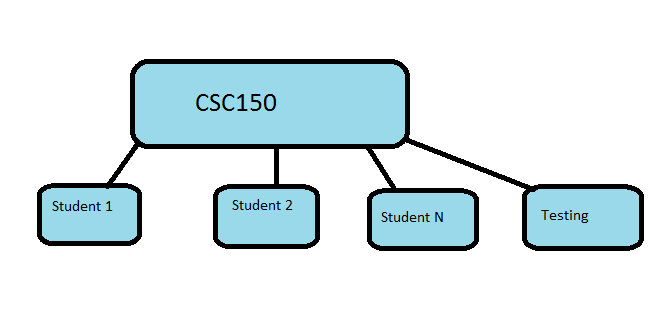
\includegraphics[width=0.75\textwidth]{./directory_structure}
\end{center}
\caption{Directory Structure \label{directory_structure}}
\end{figure}


\section{Test Setup and Execution}
Test cases were given to us by Dr. Logar.  Each one was tested and then we went through 
and manually looked at the .ans and .out files to make sure that the result in the .log file
matched with what we would actually determine the answer to be by looking ourselves.


\subsection{Test Case 1}
This test was for a student that passes all critical tests and has their program run against the rest of the test cases, no automatically generated test cases were used. This tests both the student log and class summary log file creation.

Example file structure (created using the linux tree command):


Figure~\ref{directory_tree} Shows the directory tree.

\begin{figure}[H]
\begin{center}
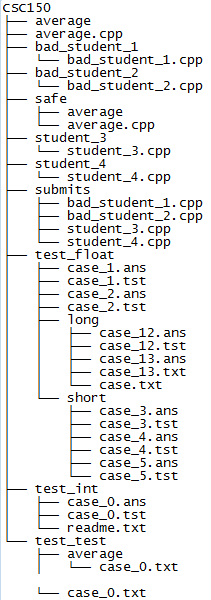
\includegraphics[width=0.25\textwidth]{./directory_tree}
\end{center}
\caption{Directory Tree \label{directory_tree}}
\end{figure}


In this test case the program is run using './grade'. It traverses to the first student directory it finds. It then compiles the cpp file within that student directory. After that, it traverses the sub-directories of CSC150 looking for files with a tst extension. It first runs the executable against all of the critical tests, designated by 'crit' in the name of the test. The executable passes all critical tests and is then run against the remaining tst files. Each test case, including critical tests, is logged in the student's log file along with the results from that test case. Once all test cases have been used, an entry in the class summary log file is made for this student along with the percentage of test cases successfully completed, excluding the critical tests. The student's log file stays within the student's directory and the class summary log file stays in the CSC150 directory.

After the program finishes running, the student log file is checked to make sure all of the critical test cases were 'PASSED' and all of the other test cases were run. Once that has been checked, the calculated percentage of tests passed is checked for accuracy. Then the class summary log is checked for the student's entry as well as the pass percentage. As long as all of those things are correct then this test case is successful.


\subsection{Additional Testing}


\begin{center}
\checkmark = Passed, x = Failed
\end{center}

\begin{table}[tbh]
\begin{center}
\begin{tabular}{| l | l | l | l |}


\hline
Test Case & Program Execution & Summary Log File & Student Log Files \\ \hline
    
   Student files and critical tests present & \multicolumn{1}{|c|}{\checkmark} & \multicolumn{1}{|c|}{\checkmark} & \multicolumn{1}{|c|}{\checkmark} \\ \hline
   
   Student files and test files present & \multicolumn{1}{|c|}{\checkmark} & \multicolumn{1}{|c|}{\checkmark} & \multicolumn{1}{|c|}{\checkmark} \\ \hline
   
   Multiple students, test files, and critical tests & \multicolumn{1}{|c|}{\checkmark} & \multicolumn{1}{|c|}{\checkmark} & \multicolumn{1}{|c|}{\checkmark} \\ \hline
   
   Float tests & \multicolumn{1}{|c|}{\checkmark} & \multicolumn{1}{|c|}{\checkmark} & \multicolumn{1}{|c|}{\checkmark} \\ \hline
   
   Int tests & \multicolumn{1}{|c|}{\checkmark} & \multicolumn{1}{|c|}{\checkmark} & \multicolumn{1}{|c|}{\checkmark} \\ \hline
   
   Students failing critical test cases & \multicolumn{1}{|c|}{\checkmark} & \multicolumn{1}{|c|}{\checkmark} & \multicolumn{1}{|c|}{\checkmark} \\ \hline
   
   Students passing all test cases & \multicolumn{1}{|c|}{\checkmark} & \multicolumn{1}{|c|}{\checkmark} & \multicolumn{1}{|c|}{\checkmark} \\ \hline
   
   Students passing critical tests but not all normal tests & \multicolumn{1}{|c|}{\checkmark} & \multicolumn{1}{|c|}{\checkmark} & \multicolumn{1}{|c|}{\checkmark} \\ \hline
   
   Generate int test cases & \multicolumn{1}{|c|}{\checkmark} & \multicolumn{1}{|c|}{N/A} & \multicolumn{1}{|c|}{N/A} \\ \hline
   
   Generate float test cases & \multicolumn{1}{|c|}{\checkmark} & \multicolumn{1}{|c|}{N/A} & \multicolumn{1}{|c|}{N/A} \\ \hline
  
   Run program w/o clearing old generated test cases & \multicolumn{1}{|c|}{\checkmark} & \multicolumn{1}{|c|}{\checkmark} & \multicolumn{1}{|c|}{\checkmark} \\ \hline
  
  Run program and clear generated test cases & \multicolumn{1}{|c|}{\checkmark} & \multicolumn{1}{|c|}{\checkmark} & \multicolumn{1}{|c|}{\checkmark} \\ \hline

\end{tabular}
\caption{System Requirements Tests Table \label{SysReqtable}}
\end{center}
\end{table}